\documentclass[11pt]{article}
\usepackage{amsmath}
\usepackage{amssymb}
\usepackage{graphicx}
\usepackage{tabularx}
\usepackage{fancyhdr}
\usepackage{lastpage}

% Page layout
\usepackage[top=1in, bottom=1in, left=1in, right=1in]{geometry}

% Header and footer
\pagestyle{fancy}
\fancyhf{}
\rfoot{Page \thepage}
\renewcommand{\headrulewidth}{0pt}

% Modified Question command with left-aligned number
\newcommand{\questiona}[2]{
    \noindent\textbf{Q#2.} #1 \hfill \textbf{[1 Mark]}
}

\newcommand{\questionb}[2]{
    \noindent\textbf{Q#2.} #1 \hfill \textbf{[2 Marks]}
}

\begin{document}

% Title section with horizontal line
\begin{center}
    \Large\textbf{GATE 2018 - Production and Industrial Engineering (PI)} \\
    \large\textbf{General Aptitude and Technical Questions} \\
    \rule{\textwidth}{0.5pt} % Horizontal line below heading
\end{center}

\vspace{0.5cm}

% General Aptitude Section
\section*{General Aptitude}

\questiona{The dress \_\_\_\_\_ her so well that they all immediately \_\_\_\_\_ her on her appearance.}{1}
\begin{enumerate}
    \item[(A)] complemented, complemented
    \item[(B)] complimented, complemented
    \item[(C)] complimented, complimented
    \item[(D)] complemented, complimented
\end{enumerate}
\vspace{0.5cm}

\questiona{The judge’s standing in the legal community, though shaken by false allegations of wrongdoing, remained \_\_\_\_\_.}{2}
\begin{enumerate}
    \item[(A)] undiminished
    \item[(B)] damaged
    \item[(C)] illegal
    \item[(D)] uncertain
\end{enumerate}
\vspace{0.5cm}

\questiona{Find the missing group of letters in the following series: BC, FGH, LMNO, \_\_\_\_\_}{3}
\begin{enumerate}
    \item[(A)] UVWXY
    \item[(B)] TUVWX
    \item[(C)] STUVW
    \item[(D)] RSTUV
\end{enumerate}
\vspace{0.5cm}

\questiona{The perimeters of a circle, a square and an equilateral triangle are equal. Which one of the following statements is true?}{4}
\begin{enumerate}
    \item[(A)] The circle has the largest area.
    \item[(B)] The square has the largest area.
    \item[(C)] The equilateral triangle has the largest area.
    \item[(D)] All the three shapes have the same area.
\end{enumerate}
\vspace{0.5cm}

\questiona{The value of the expression \( \frac{1}{1+\log_{u}vw} + \frac{1}{1+\log_{v}wu} + \frac{1}{1+\log_{w}uv} \) is \_\_\_\_\_.}{5}
\begin{enumerate}
    \item[(A)] -1
    \item[(B)] 0
    \item[(C)] 1
    \item[(D)] 3
\end{enumerate}
\vspace{0.5cm}

\questionb{Forty students watched films A, B and C over a week. Each student watched either only one film or all three. Thirteen students watched film A, sixteen students watched film B and nineteen students watched film C. How many students watched all three films?}{6}
\begin{enumerate}
    \item[(A)] 0
    \item[(B)] 2
    \item[(C)] 4
    \item[(D)] 8
\end{enumerate}
\vspace{0.5cm}

\questionb{A wire would enclose an area of 1936 m\(^2\), if it is bent into a square. The wire is cut into two pieces. The longer piece is thrice as long as the shorter piece. The long and the short pieces are bent into a square and a circle, respectively. Which of the following choices is closest to the sum of the areas enclosed by the two pieces in square meters?}{7}
\begin{enumerate}
    \item[(A)] 1096
    \item[(B)] 1111
    \item[(C)] 1243
    \item[(D)] 2486
\end{enumerate}
\vspace{0.5cm}

\questionb{A contract is to be completed in 52 days and 125 identical robots were employed, each operational for 7 hours a day. After 39 days, five-seventh of the work was completed. How many additional robots would be required to complete the work on time, if each robot is now operational for 8 hours a day?}{8}
\vspace{0.5cm}

\questionb{A house has a number which needs to be identified. The following three statements are given that can help in identifying the house number.

i. If the house number is a multiple of 3, then it is a number from 50 to 59. \\
ii. If the house number is NOT a multiple of 4, then it is a number from 60 to 69. \\
iii. If the house number is NOT a multiple of 6, then it is a number from 70 to 79.

What is the house number?}{9}
\begin{enumerate}
    \item[(A)] 54
    \item[(B)] 65
    \item[(C)] 66
    \item[(D)] 76
\end{enumerate}
\vspace{0.5cm}

\questionb{An unbiased coin is tossed six times in a row and four different such trials are conducted. One trial implies six tosses of the coin. If H stands for head and T stands for tail, the following are the observations from the four trials: 

(1) HTHTHT \hspace{1cm} (2) TTHHHT \hspace{1cm} (3) HTTHHT \hspace{1cm} (4) HHHT\_\_\_\_

Which statement describing the last two coin tosses of the fourth trial has the highest probability of being correct?}{10}
\begin{enumerate}
    \item[(A)] Two T will occur.
    \item[(B)] One H and one T will occur.
    \item[(C)] Two H will occur.
    \item[(D)] One H will be followed by one T.
\end{enumerate}
\vspace{0.5cm}

\section*{Technical Section}

\questiona{Vector triple product \( \mathbf{a} \times (\mathbf{b} \times \mathbf{c}) \) of three vectors \( \mathbf{a}, \mathbf{b} \) and \( \mathbf{c} \) is given by}{1}
\begin{enumerate}
    \item[(A)] \( (\mathbf{a} \cdot \mathbf{c})\mathbf{b} - (\mathbf{a} \cdot \mathbf{b})\mathbf{c} \)
    \item[(B)] \( (\mathbf{b} \cdot \mathbf{c})\mathbf{a} - (\mathbf{a} \cdot \mathbf{c})\mathbf{b} \)
    \item[(C)] \( (\mathbf{a} \cdot \mathbf{b})\mathbf{c} - (\mathbf{a} \cdot \mathbf{c})\mathbf{b} \)
    \item[(D)] \( (\mathbf{b} \cdot \mathbf{c})\mathbf{a} - (\mathbf{a} \cdot \mathbf{b})\mathbf{c} \)
\end{enumerate}
\vspace{0.5cm}

\questiona{A real-valued function \( y \) of real variable \( x \) is such that \( y = 5^x \). At \( x = 0 \), the function is}{2}
\begin{enumerate}
    \item[(A)] discontinuous but differentiable
    \item[(B)] both continuous and differentiable
    \item[(C)] discontinuous and not differentiable
    \item[(D)] continuous but not differentiable
\end{enumerate}
\vspace{0.5cm}

\questiona{Considering the coordinate system shown in the figure, a force of magnitude 10 kN has \( x \)-component of \(-6\) kN. Possible \( y \)-component(s) of the force is/are}{3}
\begin{center}
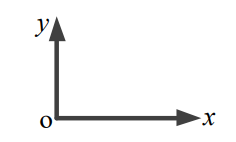
\includegraphics[width=0.4\textwidth]{figures/3.png}
\end{center}
\begin{enumerate}
    \item[(A)] +8 kN only
    \item[(B)] +5 kN only
    \item[(C)] +8 kN and \(-8\) kN
    \item[(D)] +5 kN and \(-5\) kN
\end{enumerate}
\vspace{0.5cm}

\questiona{When austenite decomposes upon cooling into two phases—ferrite and cementite, the reaction is called}{4}
\begin{enumerate}
    \item[(A)] Eutectic
    \item[(B)] Eutectoid
    \item[(C)] Peritectic
    \item[(D)] Peritectoid
\end{enumerate}
\vspace{0.5cm}

\questiona{Match the geometric tolerances with their correct symbols:
}{5}
\begin{center}
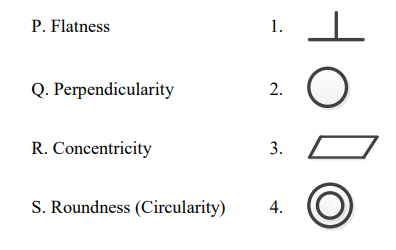
\includegraphics[width=0.6\textwidth]{figures/5.png}
\end{center}
\begin{enumerate}
    \item[(A)] P – 1, Q – 3, R – 4, S – 2
    \item[(B)] P – 3, Q – 1, R – 4, S – 2
    \item[(C)] P – 3, Q – 1, R – 2, S – 4
    \item[(D)] P – 3, Q – 2, R – 1, S – 4
\end{enumerate}
\vspace{0.5cm}

\questiona{Which one of the following instruments makes use of the principle of interference of light?}{6}
\begin{enumerate}
    \item[(A)] Optical flat
    \item[(B)] Auto-collimator
    \item[(C)] Optical projector
    \item[(D)] Coordinate measuring machine
\end{enumerate}
\vspace{0.5cm}

\questiona{In ASME process chart, the symbol \( \Box \) represents}{7}
\begin{enumerate}
    \item[(A)] operation
    \item[(B)] inspection
    \item[(C)] delay
    \item[(D)] transport
\end{enumerate}
\vspace{0.5cm}

\questiona{Which one of the following is the most appropriate control chart for measuring the variability of individual readings within a sample?}{8}
\begin{enumerate}
    \item[(A)] \( \bar{X} \)-chart
    \item[(B)] R-chart
    \item[(C)] p-chart
    \item[(D)] c-chart
\end{enumerate}
\vspace{0.5cm}

\questiona{The machines and auxiliary facilities are located according to processing sequence of the product (produced in very large quantities) in}{9}
\begin{enumerate}
    \item[(A)] Process Layout
    \item[(B)] Fixed Position Layout
    \item[(C)] Product Layout
    \item[(D)] Cellular Layout
\end{enumerate}
\vspace{0.5cm}

\questiona{Which one of the following defects is \textbf{NOT} associated with the casting process?}{10}
\begin{enumerate}
    \item[(A)] Hot tear
    \item[(B)] Porosity
    \item[(C)] Blister
    \item[(D)] Central burst
\end{enumerate}
\vspace{0.5cm}

\questiona{In an oxy-acetylene gas welding process, oxygen and acetylene are mixed in a ratio of 1.5:1 (by volume). The flame is}{11}
\begin{enumerate}
    \item[(A)] neutral
    \item[(B)] carburizing
    \item[(C)] reducing
    \item[(D)] oxidizing
\end{enumerate}
\vspace{0.5cm}

\questiona{Each of three firms P, Q and R manufactures 100 lakh components. The number of defective components produced by P, Q and R are 30, 42 and 47, respectively. The firm(s) in conformance with Six Sigma standard is/are}{12}
\begin{enumerate}
    \item[(A)] only P
    \item[(B)] P and Q
    \item[(C)] P, Q and R
    \item[(D)] Q and R
\end{enumerate}
\vspace{0.5cm}

\questiona{To make holes of 0.5 mm diameter and 30 mm depth in a mild steel component, the most suitable process is}{13}
\begin{enumerate}
    \item[(A)] chemical machining
    \item[(B)] electrochemical machining
    \item[(C)] abrasive jet machining
    \item[(D)] plasma arc machining
\end{enumerate}
\vspace{0.5cm}

\questiona{Which one of the following processes is \textbf{NOT} used for producing powders?}{14}
\begin{enumerate}
    \item[(A)] Atomization
    \item[(B)] Ball milling
    \item[(C)] Sintering
    \item[(D)] Electrolysis
\end{enumerate}
\vspace{0.5cm}

\questiona{The process in which molten thermoplastic is forced between rolls to produce thin sheets is called}{15}
\begin{enumerate}
    \item[(A)] blow moulding
    \item[(B)] compression moulding
    \item[(C)] calendering
    \item[(D)] extrusion
\end{enumerate}
\vspace{0.5cm}

\questiona{The diagonal elements of a 3-by-3 matrix are \(-10\), 5 and 0, respectively. If two of its eigenvalues are \(-15\) each, the third eigenvalue is \_\_\_\_\_.}{16}
\vspace{0.5cm}

\questiona{Weights (in kg) of six products are 3, 7, 6, 2, 3 and 4. The median weight (in kg, up to one decimal place) is \_\_\_\_\_.}{17}
\vspace{0.5cm}

\questiona{The probabilities of occurrence of events \( F \) and \( G \) are \( P(F) = 0.3 \) and \( P(G) = 0.4 \), respectively. The probability that both events occur simultaneously is \( P(F \cap G) = 0.2 \). The probability of occurrence of at least one event \( P(F \cup G) \) is \_\_\_\_\_.}{18}
\vspace{0.5cm}

\questiona{A flywheel in the form of a solid circular disc of radius 100 mm and uniform thickness has a mass of 10 kg. If it is rotating at a uniform angular velocity of 20 rad/s, the kinetic energy (in J) of the flywheel is \_\_\_\_\_.}{19}
\vspace{0.5cm}

\questiona{A cylindrical wooden block of length 50 cm is floating in water in such a way that its axis is vertical. The densities of wood and water are 800 kg/m\(^3\) and 1000 kg/m\(^3\), respectively. The submerged depth, i.e., depth of immersion (in cm) of the cylinder is \_\_\_\_\_.}{20}
\vspace{0.5cm}

\questiona{A machine consists of three components P, Q and R connected serially. The reliabilities of P, Q and R are 0.97, 0.86 and 0.93, respectively. To increase the reliability of the machine, two additional stand-by units of Q are attached. The overall reliability (up to two decimal places) of the machine is \_\_\_\_\_.}{21}
\vspace{0.5cm}

\questiona{The mean time between failures of a machine is 400 hour. If the availability of the machine is 80\%, the mean time to repair (in hour) is \_\_\_\_\_.}{22}
\vspace{0.5cm}

\questiona{Processing times on a single machine for 3 jobs are given below. All the jobs are available at time \( t = 0 \).\\

\begin{tabular}{|c|c|c|c|}
\hline
Job & 1 & 2 & 3 \\
\hline
Processing time (minute) & 15 & 3 & 6 \\
\hline
\end{tabular}\\

The mean flow time (in minute) as per the shortest processing time (SPT) sequence is \_\_\_\_\_.}{23}
\vspace{0.5cm}

\questiona{In a two-pass wire drawing process, there is a 40\% reduction in wire cross-sectional area in 1st pass and further 30\% reduction in 2nd pass. The overall reduction (in percentage) is \_\_\_\_\_.}{24}
\vspace{0.5cm}

\questiona{A double-start thread with a pitch of 2 mm is to be cut using a lathe machine. The pitch of the leadscrew of the lathe is 6 mm. The job rotates at 60 revolution per minute (RPM). The RPM of the leadscrew is \_\_\_\_\_.}{25}
\vspace{0.5cm}

\questionb{Consider the analytic function \( f(z) = x^2 - y^2 + ixy \) of the complex variable \( z = x + iy \), where \( i = \sqrt{-1} \). The derivative \( f'(z) \) is}{26}
\begin{enumerate}
    \item[(A)] \( 2x + 2iy \)
    \item[(B)] \( 2x + i2y \)
    \item[(C)] \( x + iy \)
    \item[(D)] \( 2x - 2iy \)
\end{enumerate}
\vspace{0.5cm}

\questionb{In order to evaluate the integral \( \int_{0}^{1} e^x \, dx \) with Simpson’s 1/3rd rule, values of the function \( e^x \) are used at \( x = 0.0, 0.5 \) and \( 1.0 \). The absolute value of the error of numerical integration is}{27}
\begin{enumerate}
    \item[(A)] 0.000171
    \item[(B)] 0.000440
    \item[(C)] 0.000579
    \item[(D)] 0.002718
\end{enumerate}
\vspace{0.5cm}

\questionb{A rigid link PQ of length 1.0 m is pinned at P. It rotates about P in a vertical plane with a uniform angular acceleration of 1.0 rad/s\(^2\). At an instant when the angular velocity of the link is 1.0 rad/s, the magnitude of total acceleration (in m/s\(^2\)) of point Q relative to point P is}{28}
\begin{enumerate}
    \item[(A)] 1.41
    \item[(B)] 1.73
    \item[(C)] 2
    \item[(D)] 2.83
\end{enumerate}
\vspace{0.5cm}

\questionb{In a shaft-hole system, the dimensions with tolerances (in mm) are as follows: \\
Shaft: \( \phi 20^{+x}_{-x} \) \hspace{0.5cm} Hole: \( \phi 20^{-y}_{-y} \) \\
where both \( x \) and \( y \) are positive real numbers. Which one of the following will provide an interference fit?}{29}
\begin{enumerate}
    \item[(A)] \( x = 0.05, y = 0.040 \)
    \item[(B)] \( x = 0.04, y = 0.035 \)
    \item[(C)] \( x = 0.04, y = 0.032 \)
    \item[(D)] \( x = 0.02, y = 0.035 \)
\end{enumerate}
\vspace{0.5cm}

\questionb{A machine is procured at a price of Rs. 47000 with a 2-year warranty. After two years, the annual maintenance cost (AMC) in Rs. is given by the formula: \\
AMC = \( 2000(i - 2)^2 \), for \( i > 2 \), where \( i \) is the number of years elapsed since the machine was purchased. \\
Neglect the scrap value of the machine, inflation, interest, etc. For minimizing the average cost, the machine should be replaced at the end of the year}{30}
\begin{enumerate}
    \item[(A)] 2
    \item[(B)] 4
    \item[(C)] 7
    \item[(D)] 10
\end{enumerate}
\vspace{0.5cm}

\questionb{In a service centre, cars arrive according to Poisson distribution with a mean of 2 cars per hour. The time for servicing a car is exponential with a mean of 15 minutes. The expected waiting time (in minutes) in the queue is}{31}
\begin{enumerate}
    \item[(A)] 10
    \item[(B)] 15
    \item[(C)] 25
    \item[(D)] 30
\end{enumerate}
\vspace{0.5cm}

\questionb{Actual and forecasted demands of a product are as follows:\\

\begin{tabular}{|c|c|c|c|c|c|}
\hline
Period & 1 & 2 & 3 & 4 & 5 \\
\hline
Actual demand & 180 & 170 & 165 & 170 & 200 \\
\hline
Forecasted demand & 190 & 190 & 190 & 190 & 190 \\
\hline
\end{tabular}\\

The forecast error measured in terms of mean absolute deviation (MAD) and mean absolute percentage error (MAPE), respectively, are}{32}
\begin{enumerate}
    \item[(A)] 13 and 7.84\%
    \item[(B)] 13 and 9.85\%
    \item[(C)] 17 and 7.84\%
    \item[(D)] 17 and 9.85\%
\end{enumerate}
\vspace{0.5cm}

\questionb{In a mass production firm, measurements are carried out on 10000 pairs of shaft and hole. The mean diameters of the shaft and the hole are 37.53 mm and 37.59 mm, respectively. The corresponding standard deviations are 0.03 mm and 0.04 mm. The mean clearance and its standard deviation (both in mm), respectively, are}{33}
\begin{enumerate}
    \item[(A)] 0.06 and 0.07
    \item[(B)] 0.06 and 0.06
    \item[(C)] 0.06 and 0.05
    \item[(D)] 0.07 and 0.01
\end{enumerate}
\vspace{0.5cm}

\questionb{A pressure die casting set-up was tested by injecting water (density 1000 kg/m\(^3\)) at a pressure of 200 bar. Mould-filling time was found to be 0.05 s. Afterwards, the actual casting is made by injecting the liquid metal (density 2000 kg/m\(^3\)) at an injection pressure of 400 bar. Neglect all losses (friction, viscous-effect, etc.). The approximate mould-filling time (in s) is}{34}
\begin{enumerate}
    \item[(A)] 0.05
    \item[(B)] 0.075
    \item[(C)] 0.1
    \item[(D)] 0.2
\end{enumerate}
\vspace{0.5cm}

\questionb{The value of the surface integral \( \iint_S (9x - 2y - z)\, \mathbf{i} \cdot \mathbf{n} \, dS \) over the surface \( S \) of the sphere \( x^2 + y^2 + z^2 = 9 \), where \( \mathbf{n} \) is the unit outward normal to the surface element \( dS \), is \_\_\_\_\_.}{35}
\vspace{0.5cm}

\questionb{Consider the differential equation \( \frac{d^2y}{dt^2} + 2y = 0 \) with initial conditions: at \( t = 0 \), \( y = 0 \) and \( \frac{dy}{dt} = 10 \). The value of \( y \) (up to two decimal places) at \( t = 1 \) is \_\_\_\_\_.}{36}
\vspace{0.5cm}

\questionb{One kg of air (that can be considered a calorically perfect gas with characteristic gas constant \( R = 287 \) J/kg-K and specific heat ratio \( \gamma = 1.4 \)) undergoes a constant-volume process from an initial static pressure of 1 bar to a final static pressure of 4 bar. The increase in entropy (in J/kg-K) of air is \_\_\_\_\_.}{37}
\vspace{0.5cm}

\questionb{If \( u = 2x^2 - 2y^2 \) and \( v = -axy \) represent the \( x \)- and \( y \)-components of the two-dimensional velocity field of an incompressible flow, the value of the constant \( a \) is \_\_\_\_\_.}{38}
\vspace{0.5cm}

\questionb{A spherical pressure vessel (made of mild steel) of internal diameter 500 mm and thickness 10 mm is subjected to an internal gauge pressure of 4000 kPa. If the yield stress of mild steel is 200 MPa, the factor of safety (up to one decimal place) is \_\_\_\_\_.}{39}
\vspace{0.5cm}

\questionb{A square cross-section wooden column of length 3140 mm is pinned at both ends. For the wood, Young’s modulus of elasticity is 12 GPa and allowable compressive stress is 12 MPa. The column needs to support an axial compressive load of 200 kN. Using a factor of safety of 2.0 in the computation of Euler’s buckling load, the minimum cross-sectional area (in mm\(^2\)) of the column is \_\_\_\_\_.}{40}
\vspace{0.5cm}

\questionb{Length, width and thickness of a plate are 400 mm, 400 mm and 30 mm, respectively. For the material of the plate, Young’s modulus of elasticity is 70 GPa, yield stress is 80 MPa and Poisson’s ratio is 0.33. When the plate is subjected to a longitudinal tensile stress of 70 MPa, the increase in the volume (in mm\(^3\)) of the plate is \_\_\_\_\_.}{41}
\vspace{0.5cm}

\questionb{In a V-thread, a wire is fitted such that it makes contact with the flank of the thread on the pitch line as shown in the figure. If the pitch \( p \) of the thread is 3 mm and the included angle is \( 60^\circ \), the diameter (in mm, up to one decimal place) of the wire is \_\_\_\_\_.}{42}
\begin{center}
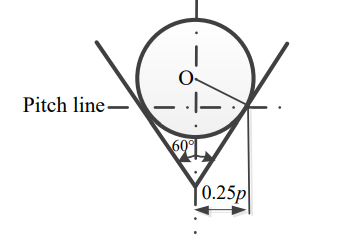
\includegraphics[width=0.5\textwidth]{figures/42.png}
\end{center}
\vspace{0.5cm}

\questionb{A project consists of three activities P, Q and R. The durations of activities follow Beta distribution. The predecessors and durations of activities are as per the following table: \\

\begin{tabular}{|c|c|c|c|c|}
\hline
Activity & Predecessors & Optimistic time (month) & Most likely time (month) & Pessimistic time (month) \\
\hline
P & — & 2 & 3 & 10 \\
Q & P & 3 & 5 & 13 \\
R & Q & 3 & 4 & 5 \\
\hline
\end{tabular} \\

The expected project completion time (in month) is \_\_\_\_\_.}{43}
\vspace{0.5cm}

\questionb{A company has two manufacturing plants (C1 and C2) and two distribution centres (D1 and D2). The capacities of C1 and C2 are 100 and 200 units, respectively. The demand for D1 and D2 are 190 and 110 units, respectively. The costs per unit (in Rs.) of transportation at different routes are as per the following matrix: \\

\begin{tabular}{|c|c|c|}
\hline
 & D1 & D2 \\
\hline
C1 & 22 & 21 \\
C2 & 20 & 27 \\
\hline
\end{tabular} \\

The minimum total cost (in Rs.) of transportation is \_\_\_\_\_.}{44}
\vspace{0.5cm}

\questionb{The annual demand of an item is 19845 units and the production rate is 100 units per day. The per-unit production cost (excluding setup cost) is Rs. 50, the per-unit holding cost is Rs. 10 per year and setup cost is Rs. 520 per setup. To minimize the total annual cost, the optimum quantity to be produced per setup is \_\_\_\_\_.}{45}
\vspace{0.5cm}

\questionb{A production line operates 7 hours a day in a 5-day week. The processing times for various job elements are as follows: \\

\begin{tabular}{|c|c|c|c|c|c|}
\hline
Job element & p & q & r & s & t \\
\hline
Processing time (s) & 5 & 10 & 12 & 3 & 15 \\
\hline
\end{tabular} \\

If the line is designed for an output of 8400 units per week, the theoretical minimum number of work stations required is \_\_\_\_\_.}{46}
\vspace{0.5cm}

\questionb{In a work sampling study of a worker, the information available are as follows: total time of study: 30 hour, number of items produced: 320, total number of observations: 1000, number of observations when worker is found working: 850 and average performance rating: 105\%. Company policy is to give allowance of 10\% of total time on the job. The standard time (in minute per item, up to one decimal place) for manufacturing the item is \_\_\_\_\_.}{47}
\vspace{0.5cm}

\questionb{The breakeven point of a manufacturing company is 50000 units. The fixed cost is Rs. 200000 and the variable cost per unit is Rs. 20. The selling price per unit (in Rs.) of the product at this breakeven point is \_\_\_\_\_.}{48}
\vspace{0.5cm}

\questionb{A 10 mm thick plate is rolled to 7 mm thickness in a rolling mill using 1000 mm diameter rigid rolls. The neutral point is located at an angle of 0.3 times the bite angle from the exit. The thickness (in mm, up to two decimal places) of the plate at the neutral point is \_\_\_\_\_.}{49}
\vspace{0.5cm}

\questionb{A cylindrical workpiece is turned at a feed of 0.1 mm/rev with a perfectly sharp tool. In ASA system, the side and end cutting edge angles are \(15^\circ\) and \(5^\circ\), respectively, as shown in the figure. The peak-to-valley roughness (in µm, up to one decimal place) of the machined surface is \_\_\_\_\_.}{50}
\begin{center}
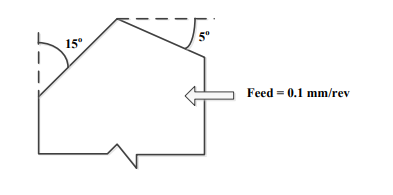
\includegraphics[width=0.5\textwidth]{figures/50.png}
\end{center}
\vspace{0.5cm}

\questionb{The worktable in a CNC machine is driven by a leadscrew with a pitch of 2 mm. The leadscrew is directly coupled to a stepper motor of step angle \(1.8^\circ\). The number of pulses required to move the worktable by 50 mm is \_\_\_\_\_.}{51}
\vspace{0.5cm}

\questionb{During orthogonal machining of a job at a cutting speed of 90 m/min with a tool of \(10^\circ\) rake angle, the cutting force and thrust force are 750 N and 390 N, respectively. Assume a shear angle of \(35^\circ\). The power (in W) expended for shearing along the shear plane is \_\_\_\_\_.}{52}
\vspace{0.5cm}

\questionb{In an electrochemical machining of aluminium with plane parallel electrodes, the current density is 70 A/cm\(^2\). Cross-sectional area of each electrode is 3 cm\(^2\). The current efficiency (i.e., the fraction of current used for dissolution of metal) is 80\%. Gram atomic weight, valency and density of aluminium are 27 gram, 3 and 2700 kg/m\(^3\), respectively. Take Faraday’s constant as 96500 Coulomb. The volumetric material removal rate (in mm\(^3\)/min) is \_\_\_\_\_.}{53}
\vspace{0.5cm}

\questionb{Two metallic sheets are spot welded by passing a current of 8000 A for 0.2 s. Assume that a cylindrical nugget of 8 mm diameter and 3 mm depth is formed. The density of the nugget is 7500 kg/m\(^3\), effective resistance of the total system is 222 micro-Ohm and heat required to produce 1.0 gram of nugget is 1400 J. The percentage of heat actually utilized in producing the nugget is \_\_\_\_\_.}{54}
\vspace{0.5cm}

\questionb{In a planar 2-degree-of-freedom robot, Link 1 of 30 cm length is connected to base by a revolute joint and Link 2 of length 20 cm is connected to Link 1 with a revolute joint as shown in the figure. The work-envelope area (in cm\(^2\)), covered by point P, is \_\_\_\_\_.}{55}
\begin{center}
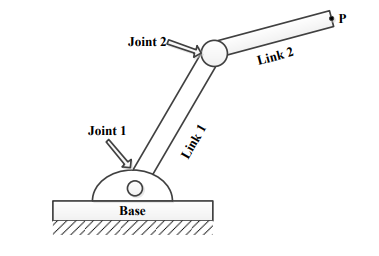
\includegraphics[width=0.5\textwidth]{figures/55.png}
\end{center}
\vspace{0.5cm}

\vspace{5cm}
\begin{center}
\textbf{END OF THE QUESTION PAPER}\\
\rule{\textwidth}{0.5pt} 
\end{center}

\end{document}